\documentclass[review]{siamart}

% 1. Preamble and packages
\usepackage{lipsum}
\usepackage{amsfonts}
\usepackage{graphicx}
\usepackage{algorithmic}
\usepackage{amsopn}
\usepackage{booktabs}

% 2. Paper title
\newcommand{\TheTitle}{%
The Multilevel Summation Method: A Python Implementation
}

% 3. Your Name
\newcommand{\TheName}{%
  Josh Bevan
}

% 4. Your Email
\newcommand{\TheAddress}{\email{%
    jjbevan2@illinois.edu
}}

% ---------------------------------------------
% ---------------------------------------------
\author{\TheName\thanks{\TheAddress}}
\title{{\TheTitle}}
\headers{\TheTitle}{\TheName}
\ifpdf%
\hypersetup{%
  pdftitle={\TheTitle},
  pdfauthor={\TheName}
}
\fi

\begin{document}

\maketitle

\vspace{1cm}
% ---------------------------------------------
% ---------------------------------------------

% [20 of 100] Problem Statement
%   - What is the problem/method/application that you are studying?
%   - Why is this important or interesting?
%   - What are a few related concepts?  (This does not need to be an exhaustive literature survey -- but some context is necessary)
%   - What are the details of the problem/method/application (enough to make a convincing case that you know what you're doing)
% [20 of 100] Approach
%   - How will you study this problem?
%   - If it's a method you're studying, what are you testing and why?
%   - If it's an application that you're studying, what method(s) will you use and why?
% [30 of 100] Numerical Results
%   - Show some numerical results.
%   - Discussion the numerical results.
%   - Show that you understand the numerical results.
%   - Did make sensible numerical tests?
% [10 of 100] Concluding remarks
%   - Critique the methods that you employed.
%   - What worked well?
%   - What did not?
%   - What would you like to do with more time?
% [10 of 100] General readability and presentation
%   - Did you use clean, easy-to-read figures?
%   - Was your write-up easy-to-follow?
%   - Was your write-up less than or equal to 8 pages (including figures/references)?
%   - Did you make a convincing case?
% [10 of 100] Code
%   - Did you include code and did your code execute what you claim?
%
% [100 of 100] Total

\section{Problem Statement}\label{sec:problem}
-Multilevel summation method\cite{2}: Efficient method for evaluation of long-range interactions in $n$-body type problems. Traditionally used to calculate forces in molecular dynamics simulations.

-MSM important because permits linear time algorithm for evaluation. Traditionally FFT used, efficient but requires periodic domain; results in unwanted interactions from copies of domain in surrounding periodic repeats.

-Algorithm has similar structure/idea to multigrid v-cycle approaches: smoothing, restriction of smooth part to coarser grid, evaluation of new short range interactions (repeat until coarsest level), then interpolation of smooth parts back down cycle until finest level\cite{1}.

\section{Approach}\label{sec:main}
-Implement main parts of algorithm in Python: smooth part separation, restriction, short-range interaction, interpolation.

-For simplicity a serial implementation will be used.

-After implementation will test various random charge distributions with increasing number of charges to evaluate scaling performance for number of bodies.

\section{Numerical Results}\label{sec:num}
Smoothing (separation of short/long-distance parts of interaction) is first part of numerics being worked on currently.

-Example plot of smoothing implementation:
\begin{figure}[!htb]
\centering
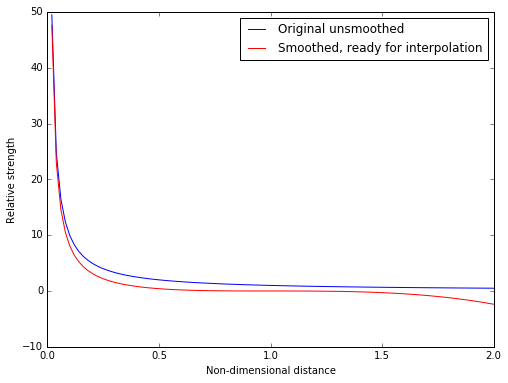
\includegraphics[width=0.6\textwidth]{smooth.PNG}
\caption{\label{fig:unrolled}Comparison of original and smoothed interaction for a single particle.}
\end{figure}

-Uses same smoothing approach as described in 2015 Hardy paper \cite{1}.

\section{Conclusions}\label{sec:conc}

\begin{thebibliography}{3}
\bibitem{1}
 David J. Hardy, Zhe Wu, James C. Phillips, John E. Stone, Robert D. Skeel, and Klaus Schulten. Multilevel Summation Method for Electrostatic Force Evaluation. Journal of Chemical Theory and Computation 2015 11 (2), 766-779 DOI: 10.1021/ct5009075
\bibitem{2}
Hardy, D. J. Multilevel summation for the fast evaluation of forces for the simulation of biomolecules. Ph.D. thesis, University of Illinois at Urbana−Champaign, Champaign, IL, 2006; Also Department of Computer Science Report No. UIUCDCS-R-2006-2546, May 2006.
\end{thebibliography}

\end{document}
